\documentclass[12pt]{article}
\usepackage{fullpage}
\usepackage{titlesec}
\usepackage{tikz}
\usepackage{amsfonts,amssymb}
\usepackage{amsmath}
\usepackage{comment}
\usetikzlibrary{automata, positioning}

\input ../libraries/mac.tex
\input ../libraries/mathmac.tex

\begin{document}
\pagestyle{plain}
\titleformat{\subsection}[runin]
  {\normalfont\large\bfseries}{\thesubsection}{1em}{}
\titleformat{\subsubsection}[runin]
  {\bfseries}{}{1em}{}

\title{Homework 6}
\author{Brooke Fugate, Michael O'Connor, Rohan Shah}
\date{}

\maketitle

\newpage
\section*{Problem B2}
\subsection*{(i)}
NFA $N_{C_G}$ for the grammer $G$:
\begin{center}
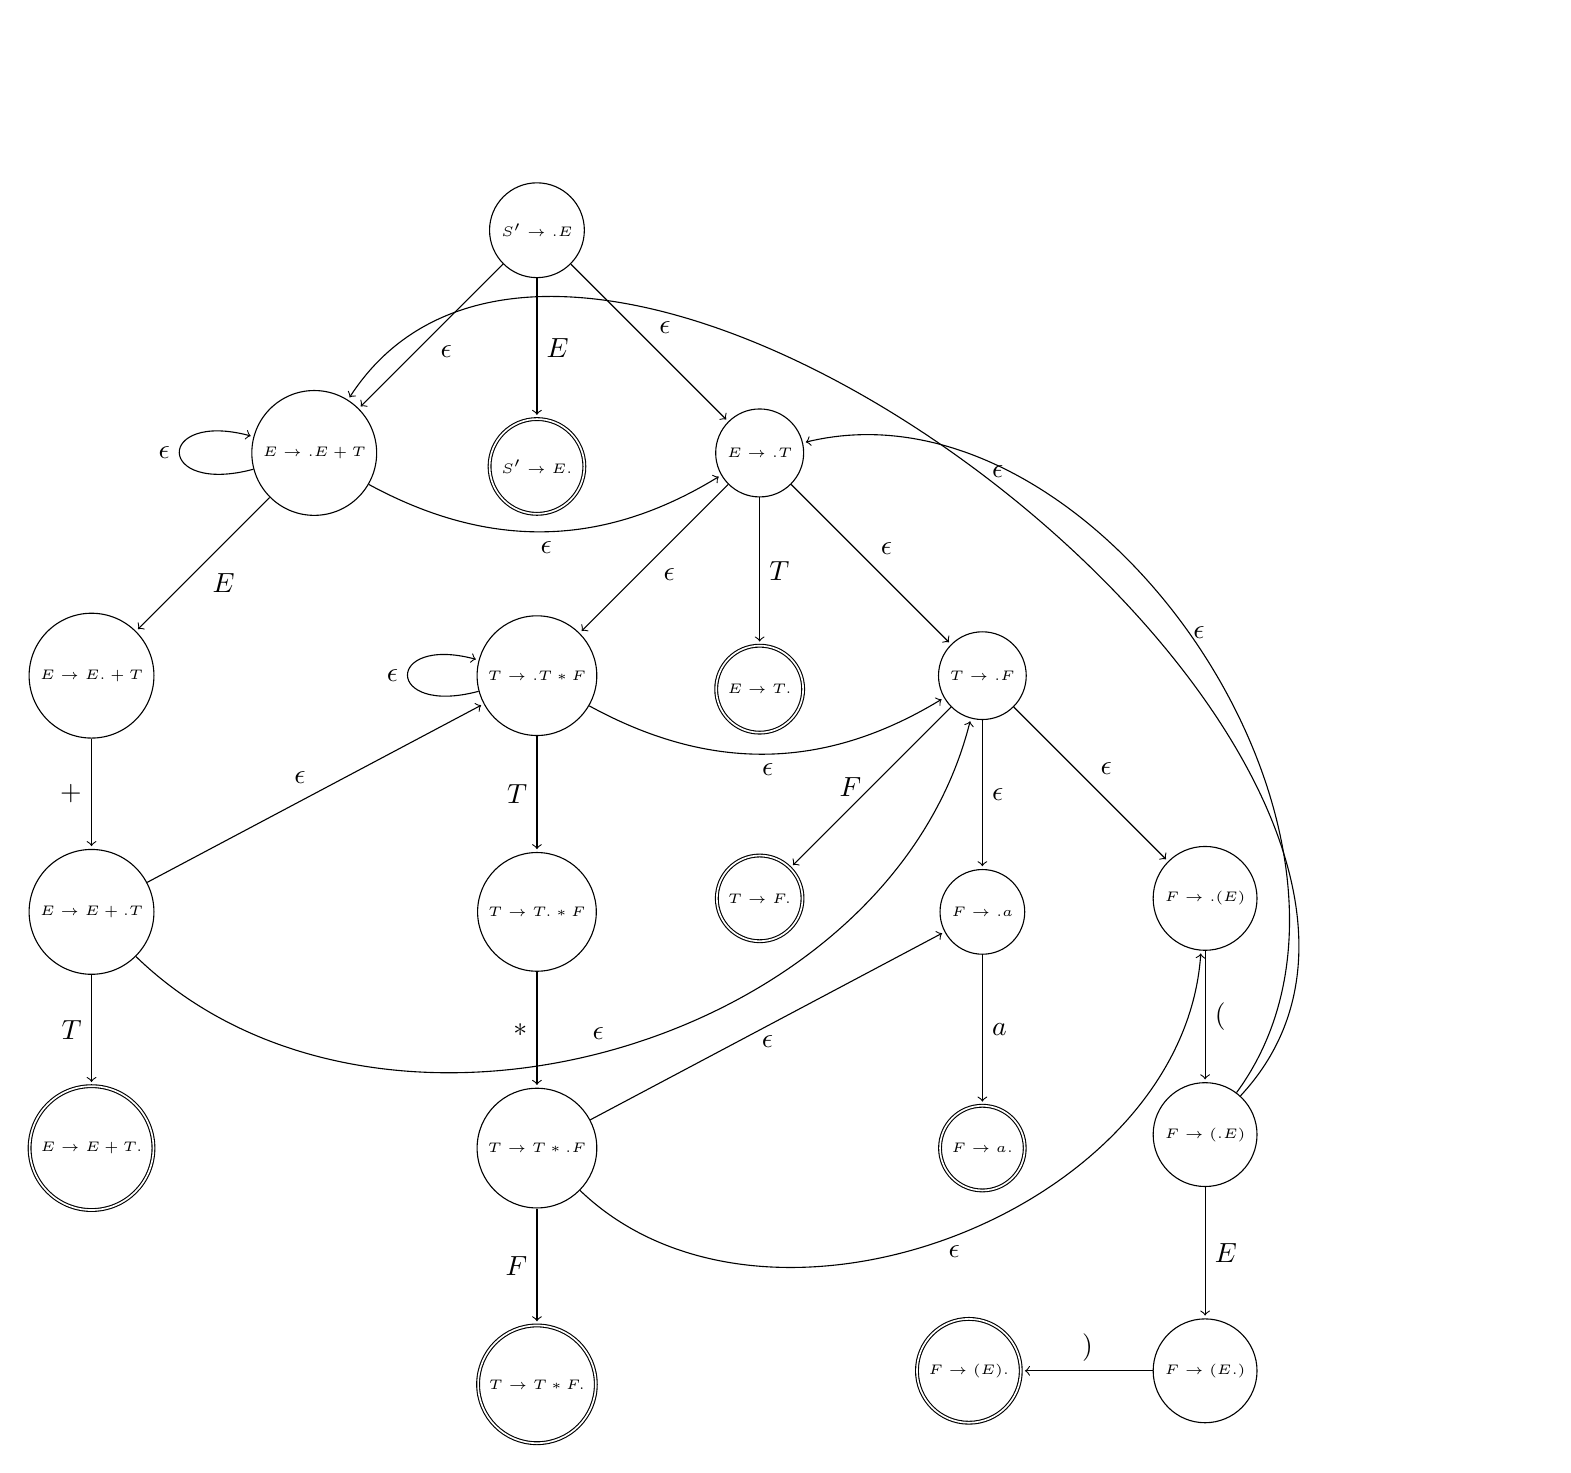
\begin{tikzpicture}[shorten >=1pt, node distance=3cm, on grid, auto]
  \node[state] (q0) {\tiny $S' \rightarrow .E$};
  \node[state, accepting] (q1) [below=of q0] {\tiny $S' \rightarrow E.$};
  \begin{scope}[node distance=4cm]
  \node[state] (q2) [below left=of q0] {\tiny $E \rightarrow .E+T$};
  \node[state] (q3) [below right=of q0] {\tiny $E \rightarrow .T$};
  \node[state] (q4) [below left=of q2] {\tiny $E \rightarrow E.+T$};
  \end{scope}
  \node[state, accepting] (q5) [below=of q3] {\tiny $E \rightarrow T.$};
  \begin{scope}[node distance=4cm]
  \node[state] (q6) [below left=of q3] {\tiny $T \rightarrow .T*F$};
  \node[state] (q7) [below right=of q3] {\tiny $T \rightarrow .F$};
  \end{scope}
  \node[state] (q8) [below=of q4] {\tiny $E \rightarrow E+.T$};
  \node[state] (q9) [below=of q6] {\tiny $T \rightarrow T.*F$};
  \node[state] (q12) [below=of q7] {\tiny $F \rightarrow .a$};
  \begin{scope}[node distance=4cm]
  \node[state, accepting] (q10) [below left=of q7] {\tiny $T \rightarrow F.$};
  \node[state] (q11) [below right=of q7] {\tiny $F \rightarrow .(E)$};
  \end{scope}
  \node[state, accepting] (q13) [below=of q8] {\tiny $E \rightarrow E+T.$};
  \node[state] (q14) [below=of q9] {\tiny $T \rightarrow T*.F$};
  \node[state] (q15) [below=of q11] {\tiny $F \rightarrow (.E)$};
  \node[state, accepting] (q16) [below=of q12] {\tiny $F \rightarrow a.$};
  \node[state, accepting] (q17) [below=of q14] {\tiny $T \rightarrow T*F.$};
  \node[state] (q18) [below=of q15] {\tiny $F \rightarrow (E.)$};
  \node[state, accepting] (q19) [left=of q18] {\tiny $F \rightarrow (E).$};

  \path[->]
  (q0) edge node {$E$} (q1)
  (q0) edge node {$\epsilon$} (q2)
  (q0) edge node {$\epsilon$} (q3)
  (q2) edge node {$E$} (q4)
  (q2) edge [loop left] node {$\epsilon$} (q2)
  (q2) edge [bend right] node [below] {$\epsilon$} (q3)
  (q3) edge node {$T$} (q5)
  (q3) edge node {$\epsilon$} (q6)
  (q3) edge node {$\epsilon$} (q7)
  (q4) edge node [left] {$+$} (q8)
  (q6) edge node [left] {$T$} (q9)
  (q6) edge [loop left] node {$\epsilon$} (q6)
  (q6) edge [bend right] node [below] {$\epsilon$} (q7)
  (q7) edge node [left] {$F$} (q10)
  (q7) edge node {$\epsilon$} (q11)
  (q7) edge node {$\epsilon$} (q12)
  (q8) edge node [left] {$T$} (q13)
  (q8) edge node {$\epsilon$} (q6)
  (q8) edge [bend right=60] node {$\epsilon$} (q7)
  (q9) edge node [left] {$*$} (q14)
  (q11) edge node {$($} (q15)
  (q12) edge node {$a$} (q16)
  (q14) edge node [left] {$F$} (q17)
  (q14) edge [bend right=65] node [below] {$\epsilon$} (q11)
  (q14) edge node [below] {$\epsilon$} (q12)
  (q15) edge node {$E$} (q18)
  (q15) edge [bend right=95] node [above] {$\epsilon$} (q2)
  (q15) edge [bend right=70] node [above] {$\epsilon$} (q3)
  (q18) edge node [above] {$)$} (q19)
  ;
\end{tikzpicture}
\end{center}

\subsection*{(ii)}
DFA $D_{C_G}$ for the grammer $G$:
\newline
\begin{tikzpicture}[shorten >=1pt, node distance=3cm, on grid, auto]
  \node[state] (0) {0};
  \node[state] (4) [below=of 0] {4};
  \begin{scope}[node distance=2cm]
  \node[state, accepting] (3) [left=of 4] {3};
  \node[state, accepting] (1) [left=of 3] {1};
  \end{scope}
  \node[state, accepting] (5) [right=of 0] {5};
  \node[state] (6) [below=of 1] {6};
  \node[state] (8) [below=of 4] {8};
  \node[state, accepting] (2) [right=of 8] {2};
  \node[state] (7) [below=of 2] {7};
  \node[state, accepting] [below=of 6] (9) {9};
  \node[state, accepting] [right=of 7] (10) {10};
  \begin{scope}[node distance=2.5cm]
  \node[state, accepting] [below=of 8] (11) {11};
  \end{scope}

  \path[->]
  (0) edge node [above] {E} (1)
  (0) edge [bend left] node {T} (2)
  (0) edge node [left] {F} (3)
  (0) edge node [left] {(} (4)
  (0) edge node {a} (5)
  (1) edge node [left] {+} (6)
  (2) edge node {*} (7)
  (4) edge node [left] {E} (8)
  (4) edge node {T} (2)
  (4) edge node [above] {F} (3)
  (4) edge [loop right] node {(} (4)
  (4) edge node [below] {a} (5)
  (6) edge node [left] {T} (9)
  (6) edge node [above] {F} (3)
  (6) edge node [below] {(} (4)
  (6) edge [bend left=100] node {a} (5)
  (7) edge node {F} (10)
  (7) edge node {(} (4)
  (7) edge [bend right] node [right] {a} (5)
  (8) edge node [left] {)} (11)
  (8) edge node {+} (6)
  (9) edge [bend right] node [below] {*} (7)
  ;
\end{tikzpicture}

\newpage
\subsection*{(iii)} Let $G$ be a reduced context-free grammar where
$G = (V,\Sigma,P,S')$ and let $C_G$ be the set of characteristic strings of $G$
defined as:
$$C_G = \{\alpha\beta \in V^* \mid S' \underset{rm}{\Longrightarrow}^* \alpha Bv
\underset{rm}{\Longrightarrow} \alpha\beta v,\ \alpha,\beta \in V^*,\ v\in
\Sigma^*,\ B \rightarrow \beta \in P \}$$
Let $N_{C_G} = (Q,\Sigma,\delta,q_0,F)$ be the NFA constructed according to the
method described in Section 1 of the handout
\textit{A Survey of LR-Parsing Methods etc.}
\medskip\newline
\textbf{Claim: } For every rightmost derivation
$$A \underset{rm}{\Longrightarrow}^* \alpha Bv \underset{rm}{\Longrightarrow}
\alpha\beta v \text{ implies } \delta^*((A \rightarrow \text{ "."}\zeta)
,\ \alpha\beta) = (B \rightarrow \beta\text{"."})$$
where $v \in \Sigma^*$, $A,B\in N$, $\alpha,\beta\in V^*$,
$(A \rightarrow \text{ "."}\zeta)\in Q$, $(B \rightarrow \beta\text{"."})\in F$
and $A \rightarrow \zeta$ is the first production in the above rightmost
derivation.
\medskip\newline
\textbf{Proof: } By induction on the length of the rightmost derivations.
\medskip\newline
For any nonterminal $A$, every rightmost derivation from $A$ is either of the form
\begin{enumerate}
\item[(i)]
$A \underset{rm}{\Longrightarrow} \zeta$,  for some  production
$A \rightarrow  \zeta$, in which case $A = B$ and $\zeta = \beta$
\item[(ii)]
$A \underset{rm}{\Longrightarrow} \lambda B_{i}\rho
\underset{rm}{\Longrightarrow}^* \lambda B_{i}w
\underset{rm}{\Longrightarrow}^* \lambda \alpha _{i}Bw_{i}w
\underset{rm}{\Longrightarrow} \lambda \alpha _{i}\beta w_{i}w$,
with $w,w_i \in \Sigma^*$, $A,B,B_i \in  N$,
$\lambda, \rho, \alpha_i, \beta\in  V^*$, and where
$$B_i \underset{rm}{\Longrightarrow} \alpha_i Bw_i
\underset{rm}{\Longrightarrow} \alpha_i \beta w_i \text{ and }
\rho \underset{rm}{\Longrightarrow}^* w.$$
\end{enumerate}

\noindent Let $B_i \rightarrow \zeta_i$ be the first production applied
in the rightmost derivation from $B_i$.
In the first case, there is a computation in $N_{C_G}$ from
state $A \rightarrow  \text{"."}\zeta$
to the final state $A \rightarrow \zeta \text{"."}$
(where again, $A \rightarrow \zeta = B \rightarrow \beta$),
and in the second case, there is a computation in $N_{C_G}$ from state
$A \rightarrow \text{ "."}\lambda B_i \rho$
to $B_i \rightarrow \text{ "."}\zeta_i$
on input $\lambda$, and a computation from
state $B_i \rightarrow \text{ "."}\zeta_i$ to
the final state $B \rightarrow \beta\text{"."}$
on input $\alpha_i \beta$.
\medskip\newline
Therefore $C_G \subseteq L(N_{C_G})$.
\medskip\newline
\textbf{Claim: } For any state $(A \rightarrow \text{ "."}\zeta) \in Q$,

$$\delta^*((A \rightarrow \text{ "."}\zeta),\ \gamma) =
(B \rightarrow \beta\text{"."}) \in F \text{ implies }
A \underset{rm}{\Longrightarrow}^* \alpha Bv \underset{rm}{\Longrightarrow}
\alpha \beta v$$
such that, the production applied in the first
rightmost derivation step is $A \rightarrow \zeta$, and $\gamma=\alpha\beta$.
\medskip\newline
\textbf{Proof: } By induction on the number of $\epsilon$-transitions in a
computation in $N_{C_G}$
\begin{enumerate}
\item[(i)]
Either $\gamma = \zeta$  and the computation is from state
$A \rightarrow \text{ "."}\zeta$ to state $A \rightarrow \zeta\text{ "."}$
\item[(ii)]
$\zeta$ is of the form $\lambda B_i\rho$,
$\gamma$ is of the form $\lambda \alpha_i \beta$, and there is
a computation on input
$\alpha_i \beta$ from some state of the form
$B_i \rightarrow \text{ "."}\zeta_i$
to the final state $B \rightarrow \beta\text{"."}$,
and a rightmost derivation as in Claim 1.
\end{enumerate}

\noindent Therefore $L(N_{C_G}) \subseteq C_G$.
\medskip\newline
Since we have sufficiently proven that $C_G \subseteq L(N_{C_G})$
and that $L(N_{C_G}) \subseteq C_G$ it follows that $C_G = L(N_{C_G})$.

\end{document}
